\section{Artificial neural network (ANN)} \label{sec:ANN}
\subsection{Background}
Artificial neural network (ANN) is a form of a nonlinear function approximator, belonging to the class of data-driven models (\aka machine learning).
The feedformward ANN architecture was originally made of multilayer perceptron (MLP), \ie, multiple layers of fully-connected perceptrons \cite{rosenblatt1957perceptron}, as schematically depicted in Figure \ref{fig:fully_connected}.
\begin{figure}[H]
    \centering
    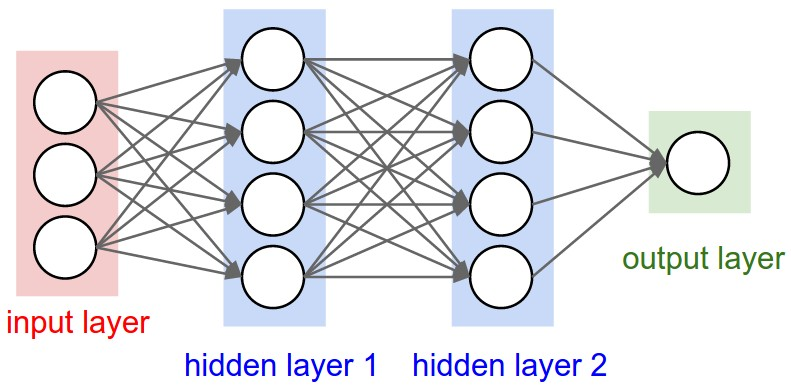
\includegraphics[width=0.6\linewidth]{../figs/related_work/fully_connected.jpeg}
    \caption{Schematics of a MLP ANN with 2 hidden layers \cite{dabbura_2022}.}
    \label{fig:fully_connected}
\end{figure}

While the ANN has evolved significantly since its first appearance in the sixties of the previous century, the same basic principles are still being used to train all its differnet variants:
\begin{enumerate}
    \item The network takes a sample of data as an input.
    \item The data is fed forward through the network's layers to eventually produce the network's output.
    \item A loss function is used to a evaluate a property of the output that is intended to be minimized.
    \item Backpropagation (an efficient algorithm for applying the chainrule of derivation) is used to calculate the loss function's partial derivatives \wrt the ANN's parameters (\aka weights).
    \item The stochastic gradient decent algorithm \cite{cauchy1847methode} uses the gradient vector of partial derivatives to  update the ANN's weights to minimize the loss function.
    \item Steps 1-5 are being repeated iteratively across different data samples and their permutations until some predefined stopping criteria is met.
\end{enumerate}

Along the years, ANNs continued to evolve in several aspects (\eg the adoption of cross-entropy loss, rectified linear units (ReLU) \cite{nair2010rectified}, \etc), but, until recently, remained somewhat unpopular compared to other machine learning methods.
In 2012, \emph{AlexNet} \cite{10.5555/2999134.2999257} an ANN achieved the best top-5 classification score on ImageNet \cite{5206848} classification contest.
Ever since, ANNs and their configurations have grown widely popular and became the SOTA solutions to a variety of real world problems in the fields of natural language processing (NLP), computer vision (CV) and many more.

\subsection{Convolutional neural network (CNN)}
In addition to the growing amount of applications to which ANNs made significant contributions, great progress was also made in the field of ANN architectures.
Among the significant advances were CNNs \cite{lecun1995convolutional}, which are built of layers of two-dimensional convolution kernels rather than perceptrons.
Convolutions are especially helpful when working with visual data, as they leverage the spatial correlation between neighboring pixels, allowing to identifying meaningful local features.
CNNs are also typically more computationally efficient, as they are made of sparse interactions between two adjacent layers \cite{Goodfellow-et-al-2016},rather than being fully-connected, and allow working with data of variable spatial dimensions.
A convolutional layer of a CNN is typically made up of 3 components:
\begin{enumerate}
    \item Convolutions: Different kernels of convolution. Their size affect the receptive field and their amount define the depth of the layer's output feature map.
    \item Normalization: A form of normalizing the layer's input to improve stability and regularity, either batchwise (\aka BatchNorm \cite{DBLP:journals/corr/IoffeS15}), per-instance (\aka InstanceNorm \cite{ulyanov2016instance}) or none at all.
    \item Activation: A non-linear function that's applied elementwise over the normalized convolution output. 
    These layers are the crucial component in allowing deep neural network to approximate extremely complex and highly-nonlinear target functions.
    Without activations, neural networks are essentially equivalent to a single linear layer, making them no more capacitated than a simple linear predictor.
    Among the common activation functions are sigmoids, hyperbolic tangent, and the ReLU discussed in the previous subsection.
    \item Pooling: A function that summarizes some statistics of neighborhoods of elements in some feature map (\eg, the average within a $2 \times 2$ rectangle neighborhood of pixels).
    Pooling results in a single scalar per neighborhood of elements, further distilling the knowledge obtained by the convolution and reducing the spatial size of its latent feature maps.
    One of the most common pooling statistics is the max-pooling \cite{Zhou1988ComputationOO}, which picks the maximum element from within each neighborhood.
\end{enumerate}

\subsection{Residual blocks}
Due to their typical structure, the more complex and nonlinear the approximated function is - the deeper the ANNs should get (there are some exceptions to that claim, but it is generally true).
However, increasing the number of layers of an ANN means that the gradients have longer paths to travel during backpropagation.
When a network becomes very deep, it typically suffers from either \emph{vanishing gradients} or \emph{vanishing gradients} \cite{bengio2013advances}, phenomena related to issues with the gradients' norms.
In 2015, He \etal \cite{DBLP:journals/corr/HeZRS15} delveloped the concept of residual blocks (\emph{ResBlocks}), where each layer of the network acted as a residual function \wrt its input layer.
ResBlocks are essentially made up of two consequent weight layers (either a fully connected or a convolutional layer) with a ReLU activation in between, followed by a summation of the ResBlock's output and input (\aka skip-connection), and finally one additional ReLU activation over the result.
A schematic depiction of a residual block can be seen in Figure \ref{fig:ResBlock}.
\begin{figure}[H]
    \centering
    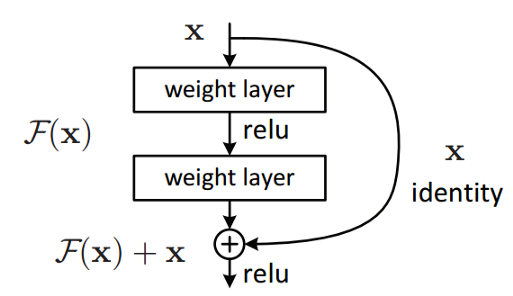
\includegraphics[width=0.7\linewidth]{../figs/related_work/residual_block.png}
    \caption{The architecture of a residual block \cite{He2016DeepRL}.} 
    \label{fig:ResBlock}
\end{figure}
By concatenating several ResBlocks together (\emph{ResNet}), He \etal managed to beat previous SOTA methods over ImageNet classification by a large margin. For the first time, it was possible to train ANNs with hundreds of layers, enabling approximation of functions with growing complexity and nonlinearity.

\subsection{Computer vision}
As mentioned before, ANNs play a significant role in the field of computer vision, and are the basis for SOTA solutions in various CV tasks.
Among the most popular CV tasks carried by ANNs are:
\begin{enumerate}
    \item Binary classification: Classifying images between two types of classes, \eg, Kaggle's dogs \vs cats challenge.
    \item Multi-class classification: Classying images between several different classes, \eg, ImageNet classification challenge where there are 1000 different classes.
    \item Semantic segmentation: Producing a per-pixel classification map rather than assigning a single label for the entire image.
    \item Object detection: Identifying a region in the image where some object appears, \eg, detecting a human face in an image. 
    Typically, the output of a detection algorithm is a rectangular bounding-box enclosing the detected object.
\end{enumerate}

One CV task of growing popularity is that of artificial data generation.
While most CV tasks take an input and produce some form of distilled information, data generation takes some input (and sometimes no input at all) and hallucinates new data.
In the domain of ANNs, there are five popular architectures that are typically used for data generation tasks:
\begin{enumerate}
    \item Variational auto-encoder (VAE) \cite{kingma2013auto}: an encoder and a decoder (essentially 2 ANNs) are trained jointly to simultaneously reconstruct an input image and minimize the Kullback-Leibler divergence \cite{csiszar1975divergence} between the distribution of the input's embedding, \ie, the feature map obtained by forward-passing the input through several hidden layers, and a normal distribution. 
    These models are usually designed to hallucinate interpolations between images belonging to the input domain rather than for transforming data to a different modality.
    \item Generative adversarial network (GAN) \cite{goodfellow2014generative}: A generator and a discriminator (again, two separate ANNs) are trained alternately with adversarial objectives. 
    The generator hallucinates an image from the target distribution that's suppose to fool the discriminator, while the discriminator attempts to classify between real images and ones that were created by the generator.
    An extensive overview about generative models will appear in the following subsection.
    \item Vision transformer (VIT) \cite{dosovitskiy2020image}: Inspired by natural language processing transformers and the attention mechanism \cite{vaswani2017attention}, VITs use both the global and local context of an input image to solve the task at hand.
    Data generation is only one of many different CV tasks tackled by VITs.
    In the region of large amounts of data, transformers are considered to outperform their counterparts.
    \item Normalizing flows \cite{rezende2015variational}: instead of implicitly training the network to transform a random sample from some probability distribution to a sample from the target domain, normalizing flows go the other way around, \ie, learn to transform the target domain to a predefined probability distribution.
    Normalizing flows utilize bijective functions as building blocks, such that the obtained transformation is invertible.
    At inference time, the inverse transformation is applied to transform a sample from the regular probability distribution to the target domain.
    \item Diffusion models\cite{sohl2015deep}: avoiding the need for a discriminator/critic, diffusion models aim to transform the prior target data distribution into random noise before revising the transformations step by step so as to rebuild a brand new sample with the same distribution as the prior.
    By some criteria, diffusion models are considered to beat GANs at generative tasks, \eg, in the work of Dhariwal \etal \cite{dhariwal2021diffusion}, where a diffusion model exhibit improved unconditional image generation results compared to SOTA GANs.

\end{enumerate}


\section{Generative adversarial newtwork}
GAN is a class of deep generative models, first introduced by Goodfellow \etal \cite{goodfellow2014generative}.
Images are the most common product of GANs, but there is no restriction in using them to produce other types of data as well.

\subsection{Architecture}
As explained in section \ref{sec:ANN}, GANs are made of a generator and a discriminator that are trained adversarially, (hopefully) until convergence.

The generator is an ANN that typically samples a random vector from some predefined probability density function, commonly Gaussian or uniform, and transforms it into an output whose dimensions match the target domain.
At initialization, the generator has no sense of the expected outcome of its transformation, and thus, assuming its weights are randomly initialized, produces a purely arbitrary output.
As training progresses, given that the discriminator generates a viable feedback, the generator adjusts its transformation to result in more authentic outputs.
The ultimate target of the generator is to fool the discriminator, \ie, to produce outputs that are indistinguishable from real data belonging to the target domain, in the "eyes" of the discriminator.

The discriminator (\aka critic in some contexts) is also an ANN, whose purpose is to discriminate between real images from the target domain and images forged by the generator.
Every sample observed by the discriminator is tagged along with a ground truth label indicating whether the image is actually real or fake (artificially generated).
    
Clearly, the better performing the generator is, the more difficult the classification task of the discriminator becomes.
Accordingly, the better the discriminator is at classifying between real and fake images, the more difficult it is for the generator to hallucinate outputs that would fool the discriminator.
This entangled setup is the reason GAN's training procedure is referred to as adversarial.
The schematics of a typical GAN are depicted in Figure \ref{fig:gan_arch}.
\begin{figure}[H]
    \centering
    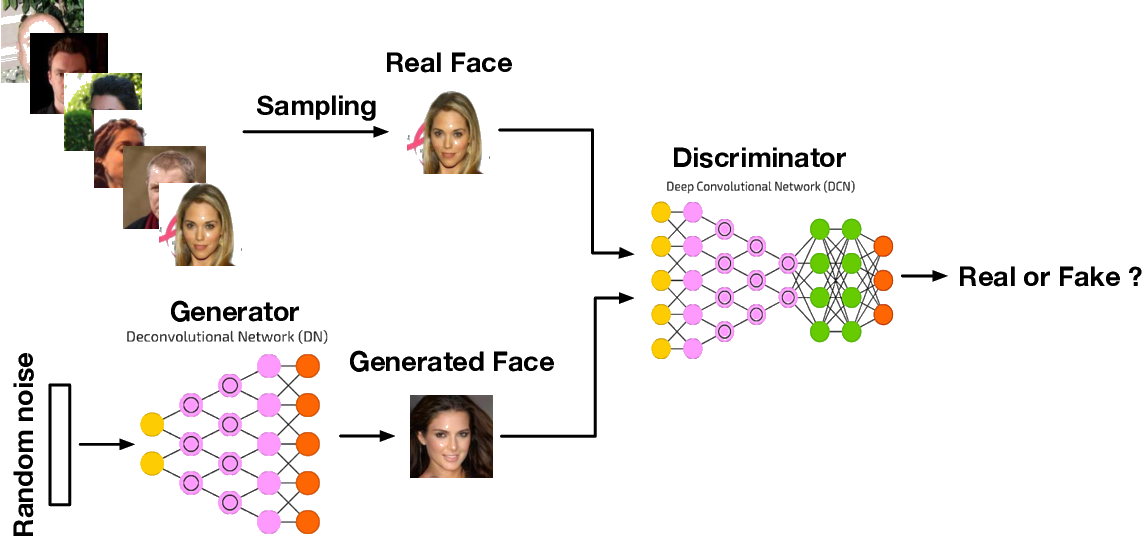
\includegraphics[width=\linewidth]{../figs/related_work/gan_arch.png}
    \caption{Schematics of a typical GAN for generating human-like faces \cite{radhakrishna_2020}.}
    \label{fig:gan_arch}
\end{figure}

\subsection{Loss function}
In the original paper, the GAN's adversarial objective function is the following:
\begin{equation} \label{eq:origGanLoss}
    \mathcal{L}(D,G) = \underset{x}{\mathbb{E}}\left[log\left(D(x)\right)\right] + \underset{z}{\mathbb{E}}\left[log\left(1 - D\left(G(z)\right)\right)\right]
\end{equation}
Where $x$ are real images from the target domain, $z$ are random vectors drawn from some predefined probability density function, $D(\cdot)$ is the discriminator's activation function (sigmoid), and $G(\cdot)$ is the generator's output.
While the discriminator attempts to maximize the objective, the generator tries to minimize it, resulting in a minimax adversarial setting ($\underset{G}{min}\underset{D}{max} \mathcal{L}(D,G)$).

In practice, it is not feasible to train both the generator and the discriminator simultaneously, as ones loss depends on the other's intrinsic parameters.
Therefore, at every iteration, one's weights are frozen while the other incurs its loss and updates its weights accordingly.
As this is the case, the generator's loss objective can be reduced to a single term:
\begin{equation}\label{eq:GanLossOnly}
    \underset{G}{min} \mathbb{E} \left[log\left(1 - D\left(G(z)\right)\right)\right]
\end{equation}
As noticed by the authers of the original paper, the loss in equation \ref{eq:GanLossOnly} tends to saturate. 
To avoid that, instead of minimizing the probability of fake classification, they proposed to instead maximize the probability of real classification:
\begin{equation}
    \underset{G}{max} \mathbb{E} \left[log\left(D\left(G(z)\right)\right)\right]
\end{equation}

While successful in several tasks, the discriminator's cross-entropy loss often results in the vanishing gradient problem described in the section \ref{sec:ANN}.
To overcome it, Mao \etal \cite{mao2017least} introduced LSGAN (Least Squares GAN) where squared error (\aka $\ell_2$ loss) is used for the discriminator's loss instead of sigmoid.
LSGAN significantly improved the generated data's quality, as well as the training stability.
More recently, Arjovsky \etal \cite{arjovsky2017wasserstein} proposed WGAN, where the earth mover (EM) distance is utilized as a loss function instead of cross-entropy or $\ell_2$.
This method assumes a 1-Lipschitzness over both generator and discriminator (sometimes enforced by gradient clipping) and is said to significantly improve stability and mitigate the notorious mode-collapse phenomenon.
Many more types of improvements to the GANs loss function were suggested along the years, but those described above were the most famous and popular ones.

\subsection{Types and applications}
Since the original GAN paper, a great deal of different types of GANs were developed for many different purposes.
Many of those developments form the underlying principles and architecture of numerous state-of-the-art models of several applications, and are way too many to cover in this mass.

Among the various tasks performed by GANs is I2I translation, where the output is conditioned on an input image.
I2I translation has a plethora of applications, such as image segmentation \cite{yang2018mri, li2020simplified}, pose estimation \cite{li2020manigan, fish2017adversarial}, colorization \cite{isola2017image, suarez2017infrared, zhang2017real}, super resolution \cite{yuan2018unsupervised, zhang2019multiple} and many more.
The I2I translation task can be roughly classified into two classes:
\begin{enumerate}
    \item Supervised / paired I2I ( I2I), where each image in the input domain has a content-aligned equivalent in the output domain. 
    \item Unsupervised / unpaired I2I (UI2I), where there are no content-equivalent pairs in the input and output domains.
\end{enumerate}
Most practical I2I tasks are performed in an unsupervised fashion, as fully registered pairs of images in two different modalities are extremely difficult to obtain.
An example of a paired \vs unpaired I2I training examples is given in Figure \ref{fig:paired_vs_unpaired}.
\begin{figure}[H]
    \centering
    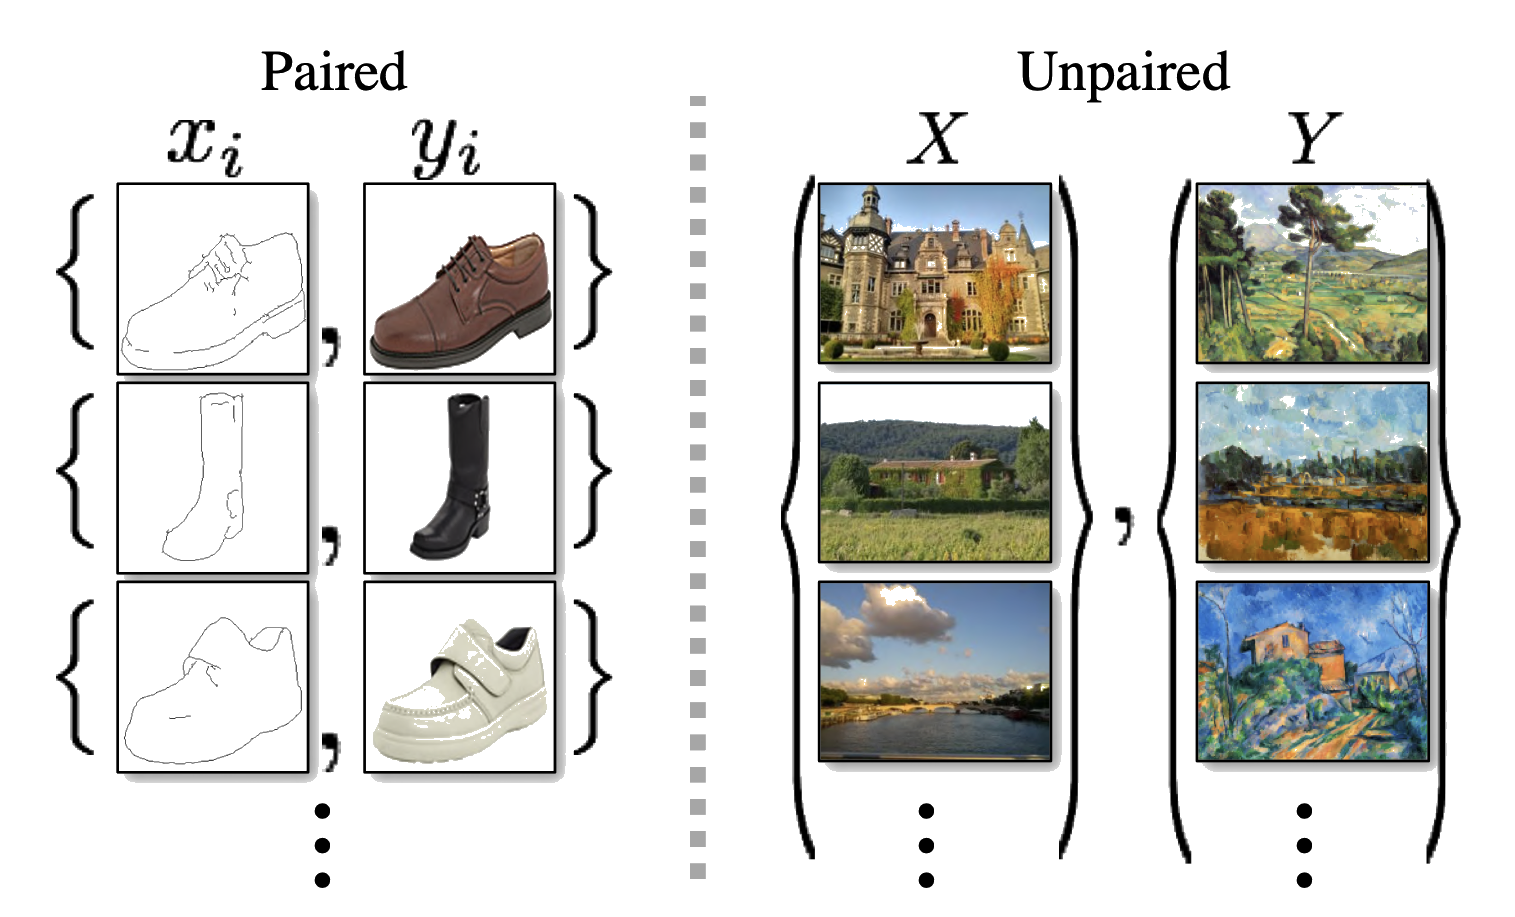
\includegraphics[width=0.75\linewidth]{../figs/related_work/paird_vs_unpaired_I2I.png}
    \caption{Paired I2I samples of sketch-to-image translation (left) \vs unpaired I2I samples of image-to-painting translation (right) \cite{CycleGAN2017}.}
    \label{fig:paired_vs_unpaired}
\end{figure}
    
The great challenge in UI2I translation is that no ground truth is available as a reference for the transformed output.
Thus, in contrast to paired I2I, pixel-level loss cannot be used to steer the training toward a better content-preserving solution.
Therefore, content preservation of the transformation must be enforced by an alternative mechanism.
The most popular strategy to ensure content preservation is to use cycle consistency \cite{Lee_2018_ECCV}.
This approach relies on two translators: one from domain A to domain B ($G_{A \rightarrow B}$), and one in the opposite direction ($G_{B \rightarrow A}$). 
Additive to the standard adversarial loss, cycle-consistency is used to penalize for discrepancies between input $x_A$ and its reconstruction by the roundtrip transformation from A to B and then back to A:
\begin{equation}
    \mathcal{L}_{cyc} = \mathcal{L}\left( x_A, G_{B \rightarrow A} \left( G_{A \rightarrow B}(x_A) \right) \right)
\end{equation}
CycleGAN \cite{CycleGAN2017}, along with DiscoGAN \cite{kim2017learning} and DualGAN \cite{yi2017dualgan} additionally impose cycle consistency over images originating in domain B, resulting in two simultaneous cyclic losses.

More cyclic-loss based extensions were suggested along the years, proposing to use a shared latent space between input and output \cite{liu2017unsupervised}, incorporating an attention module for regions of interest \cite{kim2019u} and many more.

While successfully eliminating the need for ground truth, cycle consistency inherently encourages the transformation to encode information about the input that serves solely for the purpose of cyclic reconstruction.
This encoded information comes at the expense of fidelity to the target modality, which is clearly undesirable.
In an attempt to eliminate the need for cycle consistency, several approaches have implemented a one-sided translation that manages to preserve content in a different fashion.
Typically, this is done by embedding both input and target in some shared style-agnostic space. 
The geometric distance between the embeddings is treated as a measure of content discrepancy, and then minimized to improve content preservation.
Fu \etal \cite{fu2019geometry} encouraged preservation of the geometric relationship between an input and its geometrically transformed versions and their outputs. 
Both F-LSeSim \cite{zheng2021spatially} and contrastive unpaired translation (CUT) \cite{park2020cut} used contrastive representation learning by maximizing the similarity between pairs of corresponding patches in the input and output, and minimizing it for non-matching patches.

In this thesis, we built upon the architectures of both CycleGAN and CUT.
Therefore, we provide some further attention to those model and describe them in more detail.

\subsubsection{CycleGAN}
As explained, CycleGAN \cite{CycleGAN2017} is a cycle-consistency-loss-based GAN for performing UI2I.
CycleGAN was among the first models and probably one of the most famous architectures for performing UI2I.
The loss function of CycleGAN is a weighted sum of different components:
\begin{itemize}
    \item adversarial loss (specifically, patch LSGAN loss, which calculates the least-squared GAN loss for random patches).
    \item Cycle-consistency loss, for each of A and B data domains, between an input and its reconstructed version. The authors used $\ell_1$ distance as the discrepancy measure. put in math:
    \begin{equation}
        \mathcal{L}\left( x_A, G_{B \rightarrow A} \left( G_{A \rightarrow B}(x_A) \right) \right) = 
        ||x_A - G_{B \rightarrow A} \left( G_{A \rightarrow B}(x_A) \right)||_1
    \end{equation}
    \item Identity loss, where an input of domain A is transformed by $G_{B \rightarrow A}$, as if it was an image from domain B, and compared to the original input.
    The idea behind identity loss is to minimize the effect that the generator $G_{B \rightarrow A}$ has on images from domain $A$.
    This helps mitigate color discrepancy issues that otherwise arise when applying the cycle transformation.
    The $\ell_1$ was used for the identity loss as well.
\end{itemize}
In each training iteration, the weighted loss is evaluated simultaneously for input batches from domain A and from domain B.
The schematics of the CycleGAN architecture is depicted in Figure \ref{fig:CycleGAN_loss_schematics}.
\begin{figure}[H]
    \centering
    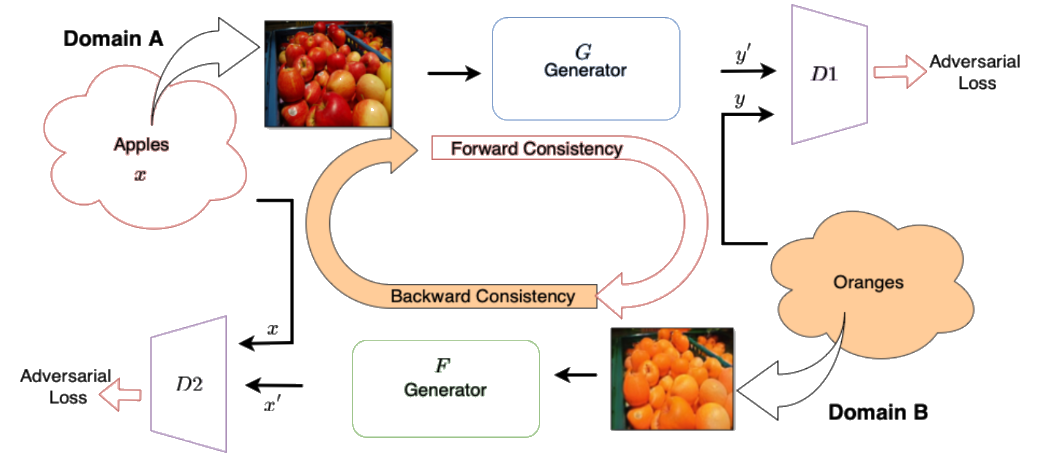
\includegraphics[width=0.8\linewidth]{../figs/related_work/CycleGAN_arch.png}
    \caption{Schematic of the CycleGAN's architecture \cite{chandhok_2022}.}
    \label{fig:CycleGAN_loss_schematics}
\end{figure}

CycleGAN was trained and utilized for several different purposes, such as horses $\rightarrow$ zebras, winter $\rightarrow$ summer, apples $\rightarrow$ oranges, \etc.
Exemplary results of the these trained translations can be observed in Figure \ref{fig:CycleGAN_results}.
\begin{figure}[H]
    \centering
    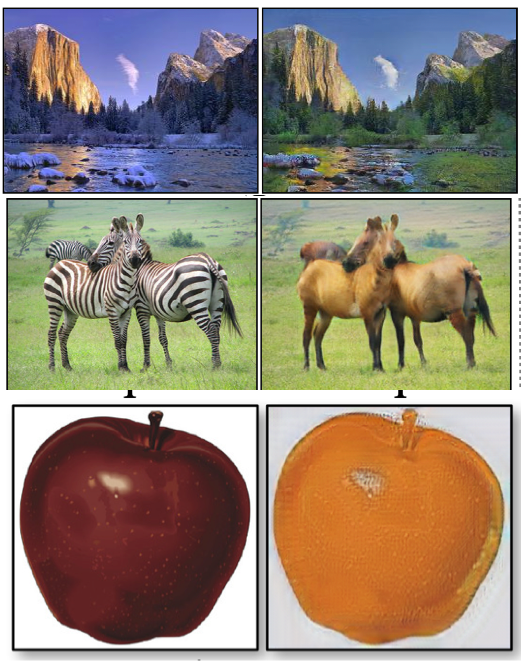
\includegraphics[width=0.3\linewidth]{../figs/related_work/CycleGAN_results.png}
    \caption{CycleGAN's exemplary results for different UI2I tasks \cite{CycleGAN2017}.}
    \label{fig:CycleGAN_results}
\end{figure}

\subsubsection{CUT}
Contrastive unpaired translation (CUT) GAN \cite{park2020cut} belongs to the family of non-cycle-consistent models for UI2I.
Many of CUT's design choices match those of CycleGAN variants (\eg, using 9 ResBlocks as the generator's backbone).
To handle the lack of cycle-consistency, an alternative patchwise contrastive loss is applied instead.
The procedure for calculating the contrastive loss is as follows:
\begin{enumerate}
    \item An input image $x$ of some domain is translated via a generator to a different domain(same as in CycleGAN):
    \begin{equation*}
        y = G(x)        
    \end{equation*}
    \item Random non-overlapping patches of the input $x$ and output $y$ are selected correspondingly, \ie, each patch of $x$ spatially corresponds to a patch in $y$.
    \item The random patches of both $x$ and $y$ are fed into the same generator ($G(\cdot)$), and prominent latent feature maps are concatenated to assemble a feature tensors $\tilde{x}$ and $\tilde{y}$.
    \item A multilayer perceptron (MLP) network is used to encode all the feature tensors into vectors in a dedicated embedding space.
    \item Cross-entropy loss is used to encourage similarity between spatially corresponding patches in $\tilde{x}$ and $\tilde{y}$, and minimize that similarity between non-corresponding patches.
    This is the contrastive loss that guarantees spatial coherency between the input and target domains, as it constraints that the generator maintains a high mutual information between activations of its input and output.
\end{enumerate}
An illustration of the patchwise contrastive loss calculation process appears in Figure \ref{fig:CUT_contrastive_sceheme}.
\begin{figure}[H]
    \centering
    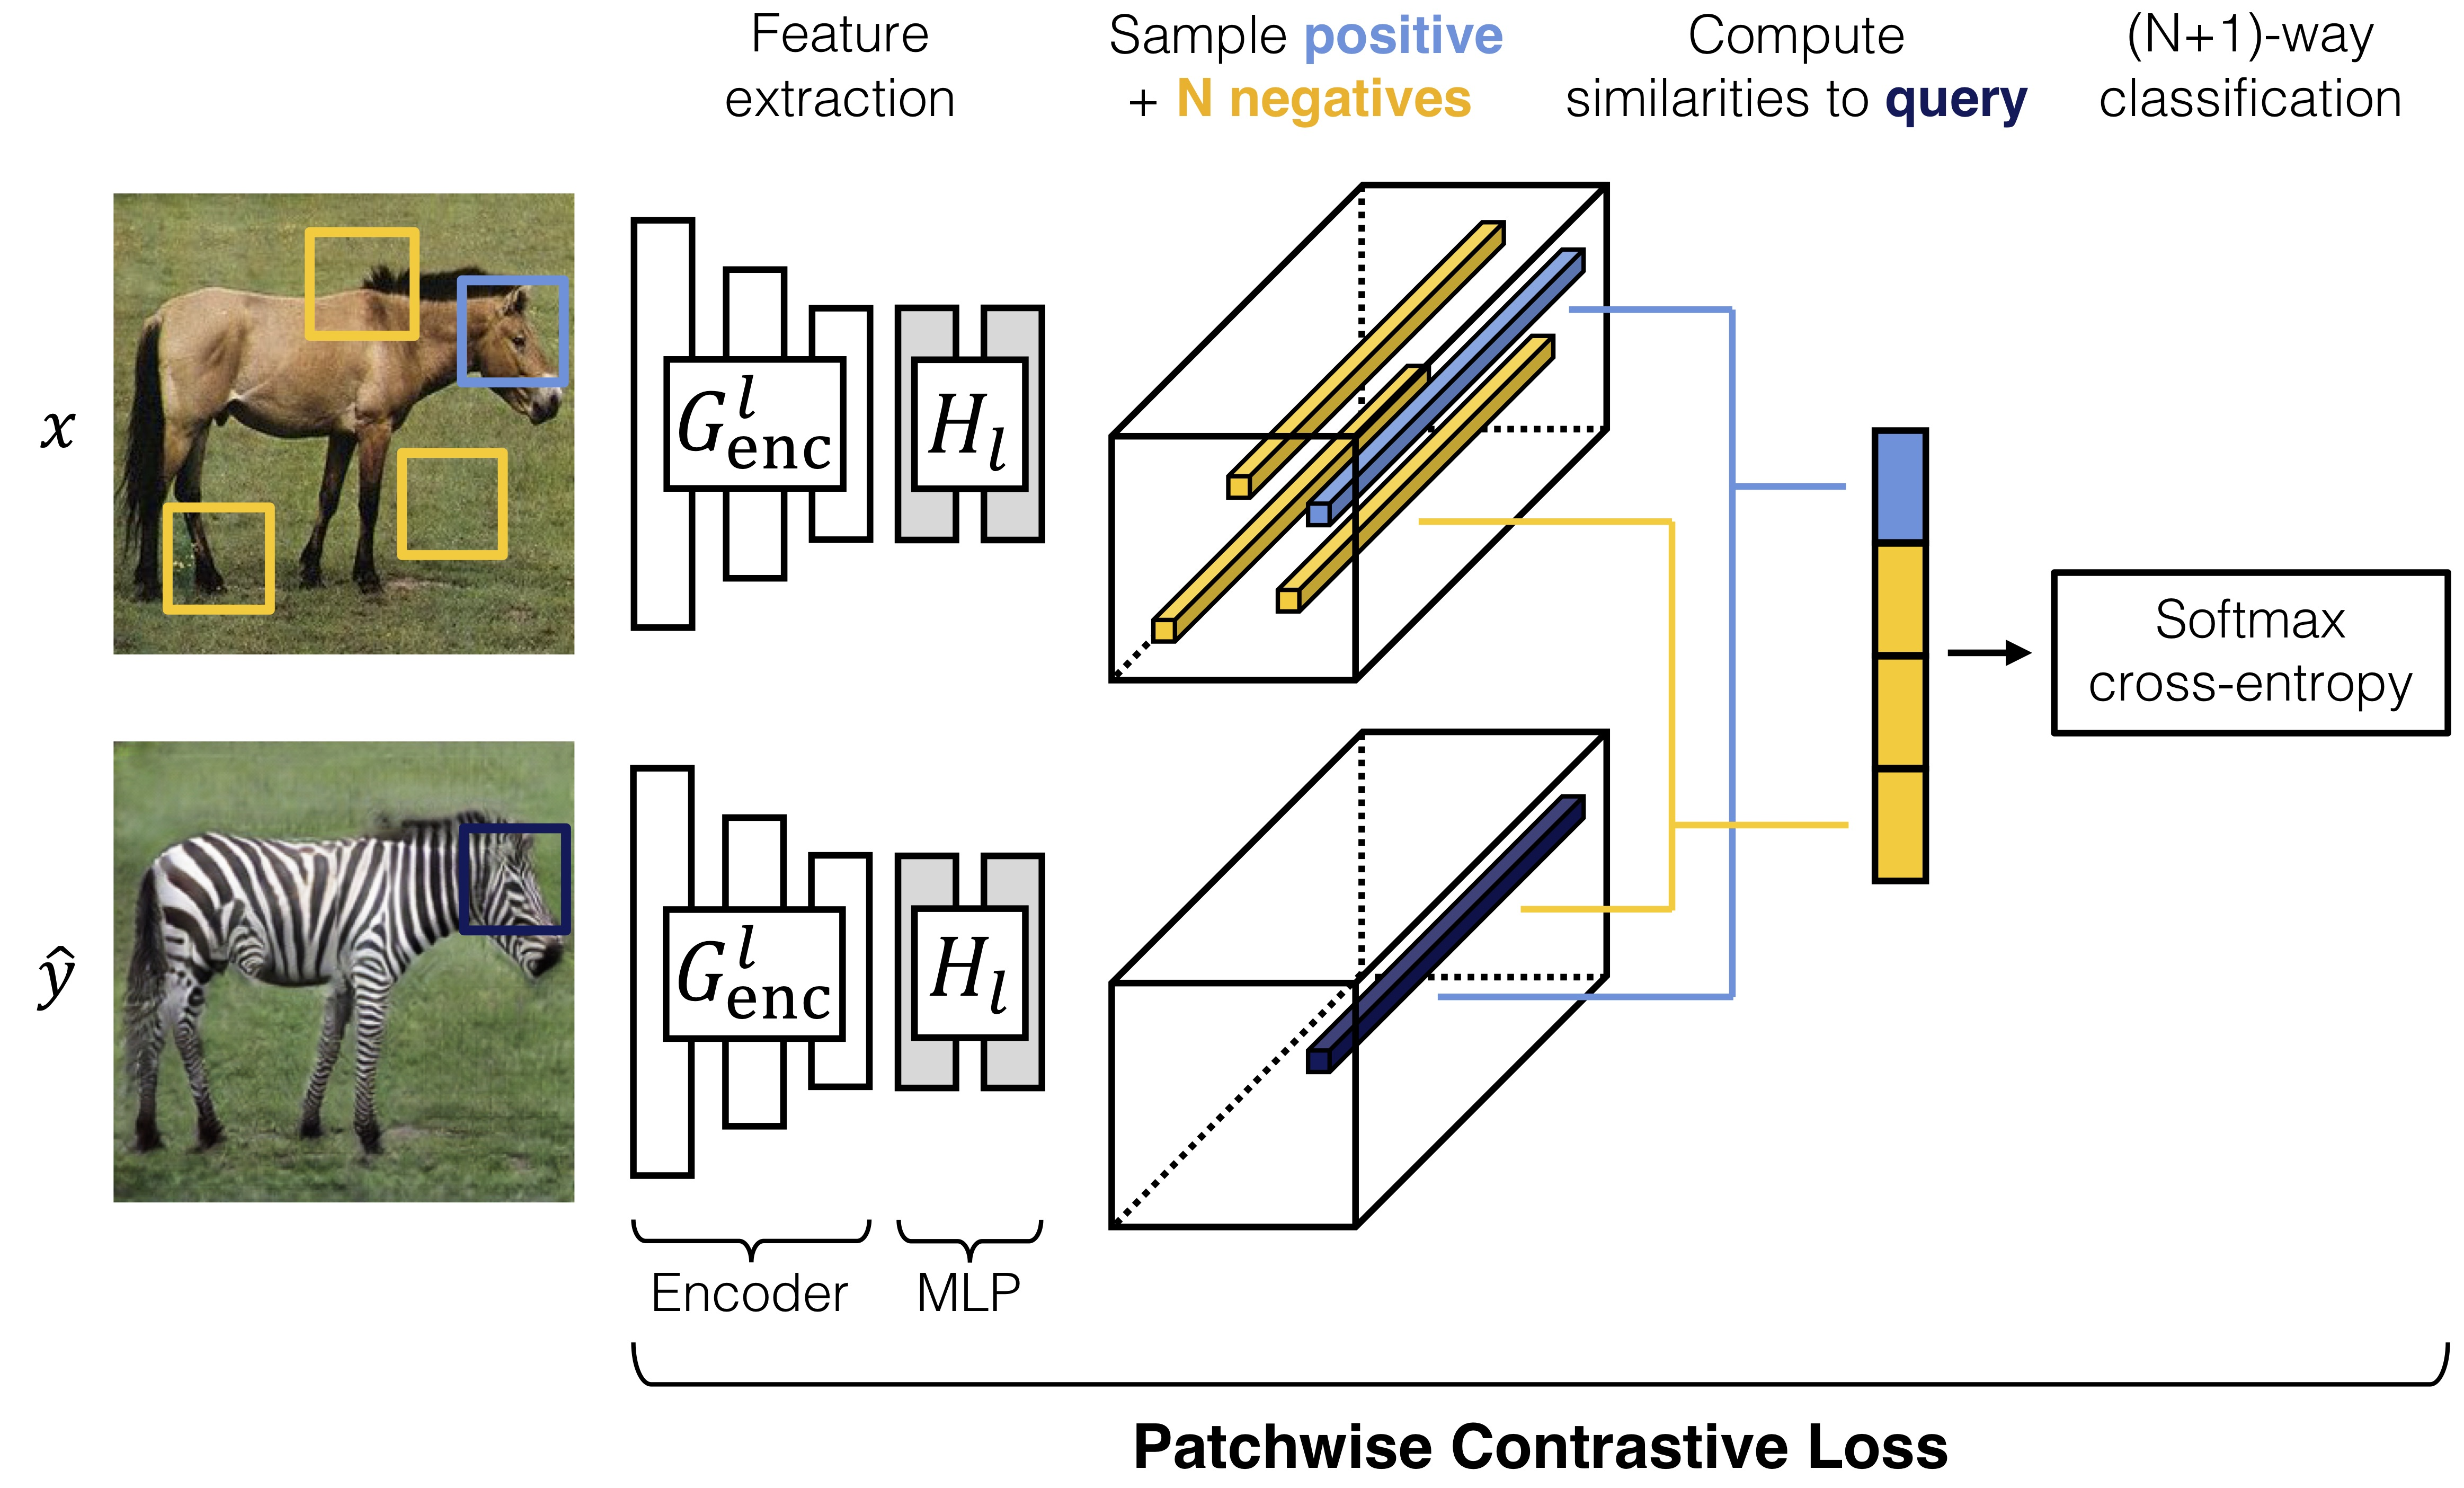
\includegraphics[width=\linewidth]{../figs/related_work/CUT_contrastive_sceheme.jpg}
    \caption{Schematic of the patchwise contrastive loss calculation procedure \cite{park2020cut}.}
    \label{fig:CUT_contrastive_sceheme}
\end{figure}    

The other loss components, \ie, adversarial loss and identity loss, were the same as in CycleGAN.
As claimed by the authors, the elimination of the second set of generator and discriminator and the cyclic reconstruction resulted in a more stable and memory efficient solution, which produces superior results to that of CycleGAN.

\section{Thermal imaging}

\subsection{Blackbody radiation}
Black-body radiation is the thermal electro-magnetic signal that is emitted by an ideal opaque object due to its temperature.
Planck's law of black-body radiation states that:
\begin{equation} \label{eq:Plancks-law}
  B_{\lambda}(T) = \frac{2\pi hc^2}{\lambda^5}\frac{1}{e^{\frac{hc}{\lambda kT}} - 1} \; \; \left[W sr^{-1} m^{-2} \mu m^{-1}\right]
\end{equation}
where $B_{\lambda}(T)$ is the ideal object's spectral radiance density, $h$ is Planck's constant, $c$ is the speed of light in a vacuum, $k$ is the Boltzmann constant, $\lambda$ is the electromagnetic wavelength and $T$ is the object's absolute temperature \cite{FundamentalsOfInfraredThermalImaging}.
As evident from Planck's law, the spectral radiance density is different depending on the object's temperature, as depicted in Figure \ref{fig:Planck_density}.
\begin{figure}[H]
  \centering
  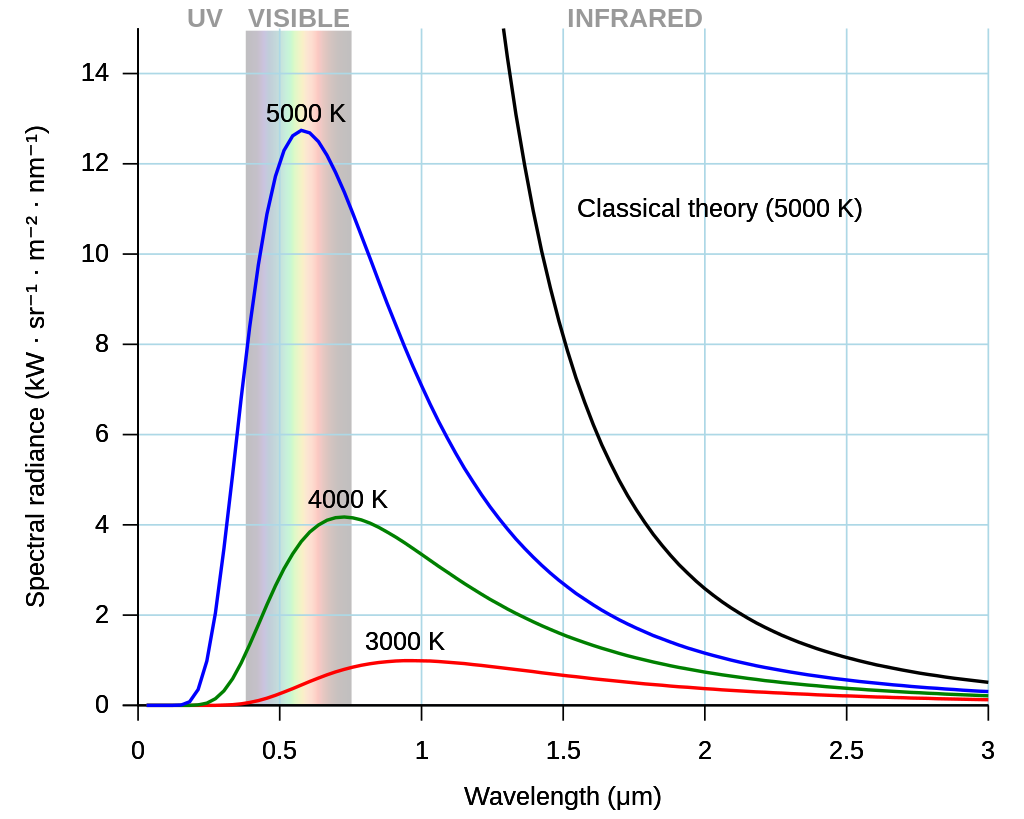
\includegraphics[width=\linewidth]{../figs/methods/planck.png}
  \caption{Planck's spectral radiance densities for different object temperatures \cite{enwiki:1128338285}.}
  \label{fig:Planck_density}
\end{figure}

The Stefan-Boltzmann law \cite{surhone2010stefan} ties the power radiated from an object (which is the result of integrating $B_{\lambda}(T)$ over the entire spectrum of wavelengths from zero to infinity) to the object's temperature:
\begin{equation} \label{eq:stephan-boltzmann-ideal}
    P(T) = \int_0^\infty B_{\lambda}(T) d\lambda = \frac{\sigma}{\pi} T^4 \; \;\left[W sr^{-1} m^{-2}\right]
\end{equation}
where $P$ is the radiated power and $\sigma$ is the Stephan-Boltzmann constant. 

A real-world opaque object emits less power than an ideal black body at the same temperature. 
The ratio between the radiation emission of an object and that of an ideal blackbody at the same temperature is called \emph{emissivity}.
The emissivity is a function of various a-priori unpredictable characteristics of the object, such as material type, surface structure, viewing angle, \etc.
Thus, the Stephan-Boltzmann law for practical objects is given by:
\begin{equation} \label{stephan-boltzmann-practical}
  P(T) =  \frac{\sigma}{\pi} \epsilon T^4 \; \; \left[W sr^{-1} m^{-2}\right]
\end{equation} 
where $\epsilon$ is the object's emissivity.
In general, the emissivity is a function of the wavelength \cite{kerekes2008spectral}, but it is used here as a constant that reflects its expected value over the thermal bandwidth for simplification.

\subsection{Microbolometric camera acquisition}
Microbolometric camera is a thermal camera who's sensor is a microbolometer, which is a thermally sensitive resistor.
According to \cite{FundamentalsOfInfraredThermalImaging}, when acquired by a thermal microbolometric camera with a finite bandwidth, the incident power on the microbolometer (the thermal camera's sensor) can be described by:
\begin{equation} \label{BolometerIncidentPower}
  \phi(T) = \gamma F_\mathit{pan} \epsilon T^4 \; \; \left[W sr^{-1} m^{-2}\right]
\end{equation}
where $\phi$ is the incident power on the microbolometer, $\gamma$ is a constant governed by the camera's geometrical properties and $F_\mathit{pan}$ represents the fraction of power that is within the camera's bandwidth.
When applying an IR bandpass filter over the camera lens, equation \ref{BolometerIncidentPower} still holds except that $F_\mathit{pan}$ is replaced by $F_\mathit{mono}$, reflecting the fraction of power that is strictly within the bandpass region of the applied filter \cite{FundamentalsOfInfraredThermalImaging}.

Since $\gamma, F_\mathit{pan}, \epsilon$ are all constants, they can be reduced into a single coefficient:
\begin{equation} \label{BolometerIncidentPowerSimplified}
  \phi(T) = a T^4 \; \; \left[W sr^{-1} m^{-2}\right]
\end{equation}
suggesting that the incident power is proportional to $T^4$.
Consequently, a thermally stabilized camera operating in radiometric mode, \ie, when the image intensity levels are linear in the incident power, the intensity of a pixel is obtained by an affine transformation of $T^4$:
\begin{equation} \label{eq:naiveAffineTrans}
  I(T) = b + a T^4
\end{equation}
where $I$ is the intensity level of the pixel and $b$ is the digital bias level. 
